\section{Применение ``CATIA-GDML geometry builder'' к CBM RICH}\label{sec:RICHgeo}

Значительная часть работы над ``Builder'' выполнялась при поддержке группы CBM RICH, поэтому самая сложная MC-модель построенная с помощью ``Builder'' это CBM RICH. Построенная за несколько итераций модель имеет достаточно сложную иерархию и характеризуется высокой степенью подробностей.

Для того, чтобы GDML без проблем импортировался в CbmRoot было написано дополнение.

Геометрическая MC-модель детектора RICH эксперимента CBM имеет многоуровневую структуру, в основном обоснованную физической структурой сборки, но иногда и \todo бывает неочевидной и неестественной с целью повышения эффективности проведения частиц.

На момент написания данной работы инженерный проект не был завершён --- некоторые узлы были проработаны достаточно подробно и прошли несколько этапов уточнения, в которых модель менялась принципиально. В то же время некоторые узлы существуют лишь на концептуальном уровне. В первую очередь к ним относится форма и конструкция корпуса детектора, проектирование которой не составляет особого труда и может быль отложена на более поздний этап. Большая часть корпуса не оказывает влияния на эффективность детектора, т.к. лежит за пределами геометрического аксептанса, поэтому допускается моделирование физики детектора с упрощённой моделью корпуса, либо вообще без него.

В детекторе RICH можно выделить несколько подсистем --- фоточувствительная камера, магнитный экран вокруг камеры, зеркала, система опор зеркал, часть ионопровода в RICH, корпус детектора. Рассмотрим реализацию каждой подсистемы в MC-модели, построенной с помощью ``CATIA-GDML geometry builder''.

\subsection{Фоточувствительная камера}\label{sec:RICHgeoCamera}

Планируется, что фоточувствительная камера CBM RICH будет составлена из модулей, содержащих 2$\times$3 МА~ФЭУ Hamamatsu H12700, см. \figref{fig:H12700drawing}. Один такой МА~ФЭУ имеет габариты 52$\times$52~мм$^2$, между МА~ФЭУ оставляется зазор 1~мм для запаса по точности, таким образом размер модуля составляет 158мм$\times$105мм.

\begin{figure}[H]
\centering
\includegraphics[width=0.7\textwidth]{pictures/H12700_drawing.png}
\caption{Чертёж МА~ФЭУ H12700 из документации.}
\label{fig:H12700drawing}
\end{figure}

В момент написания данной работы ведётся работа по проектированию модуля, разработке программ для FPGA, но имеются изготовленный прототип. Помимо МА~ФЭУ в модуль входят 12~плат передней электроники DIRICH, одна плата, обеспечивающая питание, и одна плата концентрации данных. В основе модуля лежит плата-адаптер, к которой с одной стороны подсоединяются МА~ФЭУ, а с другой --- все платы. CAD-модель и MC-модель модуля показаны на \figref{fig:geoMCmodule}.

\begin{figure}[H]
\begin{minipage}[b]{0.495\textwidth}
\includegraphics[width=1.0\textwidth]{pictures/PMTmoduleCAD.png}
\end{minipage}
\hspace{0.01\textwidth}
\begin{minipage}[b]{0.495\textwidth}
\includegraphics[width=1.0\textwidth]{pictures/Module_1_cut.png}
\end{minipage}
\caption{CAD-модель (слева) и MC-модель (справа) модуля фоточувствительной камеры CBM RICH.}
\label{fig:geoMCmodule}
\end{figure}

Иерархия объёмов, моделирующих модуль фоточувствительной камеры CBM RICH приведена на \figref{fig:Module_geoStructure}.

\begin{figure}[H]
\centering
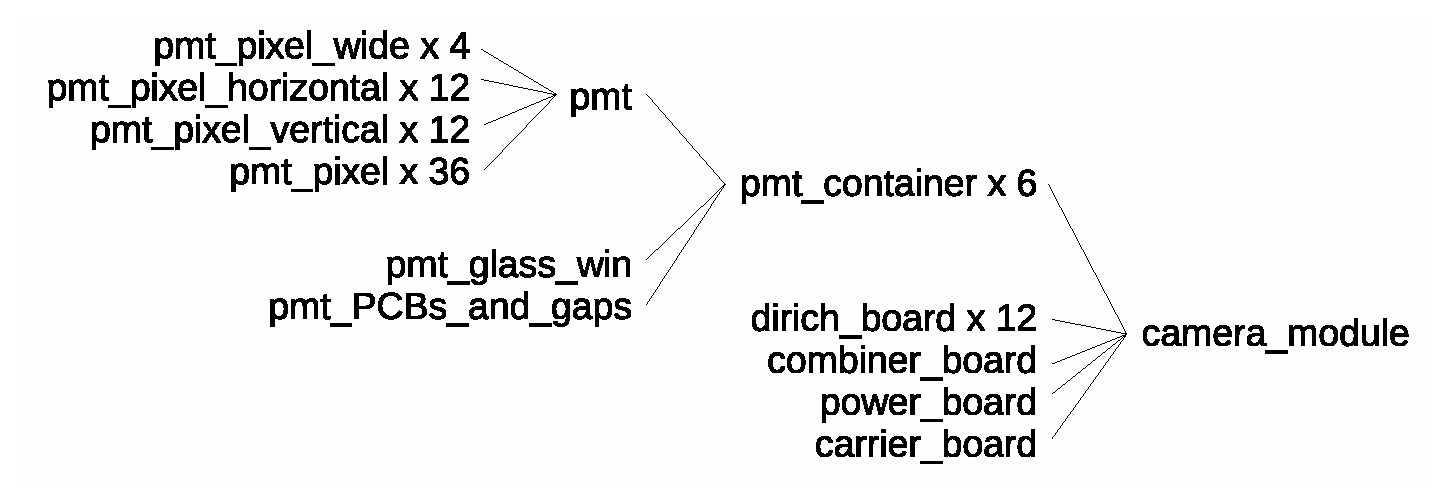
\includegraphics[width=0.7\textwidth]{pictures/Module_geoStructure.eps}
\caption{Иерархия объёмов, моделирующих модуль фоточувствительной камеры CBM RICH.}
\label{fig:Module_geoStructure}
\end{figure}

%Пиксели
%№№ 2-7, 58-63, 9, 17,..., 49, 16, 24,..., 56
МА~ФЭУ моделируется до уровня пикселей. Это позволяет максимально приблизить моделирование прохождения частиц в CbmRoot и обработку реальных данных. В соответствии с документацией, у МА~ФЭУ H12700 пиксели имеют разные размеры (см. \figref{fig:H12700drawing}): угловые пиксели (№№ 1, 8, 57, 64) 6.25мм$\times$6.25мм, пиксели по краям, кроме угловых, --- 6.25мм$\times$6мм, остальные, центральные пиксели --- 6мм$\times$6мм. Для того, чтобы представить три типа пикселей в MC-модели, необходимо три отдельных объёма, имеющих разную форму. Чтобы сделать модель максимально понятной и гибкой принято решение отделить пиксели из крайних горизонтальных рядов от пикселей из крайних вертикальных рядов и моделировать их с помощью двух разных объёмов размером 6мм$\times$6.25мм и 6.25мм$\times$6мм соответственно. Это позволит позиционировать все пиксели без поворотов.

Таким образом вводится три объёма: \volumename{pmt\textunderscore pixel\textunderscore wide} для угловых пикселей, \volumename{pmt\textunderscore pixel\textunderscore horizontal} для пикселей в крайних горизонтальных рядах, \volumename{pmt\textunderscore pixel\textunderscore vertical} для пикселей в крайних вертикальных рядах и \volumename{pmt\textunderscore pixel} для всех остальных пикселей, расположенных в центральной зоне. Все 4 объёма имеют форму примитива box с толщиной вдоль оси Z, равной 0.5мм, материал CsI, который в данный момент используется в моделировании как активный материал для фоточувствительных элементов. Толщина выбрана произвольно, она не имеет значения, т.к. из-за того, что материал объёма активный, т.е. объём объявлен чувствительным, система проведения частиц будет вырабатывать сигнал о пересечении треком границы объёма и передавать управление методу \methodname{ProcessHits} класса детектора \classname{CbmRich}. В реализации этого метода вырабатывается Point, причём физика не оказывает никакого влияния. Даже если толщина объёма слишком маленькая, чтобы произошло какое-либо взаимодействие, флаг активности обязывает систему вызвать \methodname{ProcessHits}.

Объём \volumename{pmt} соответствует части МА~ФЭУ, включающей в себя фотокатод (пиксели) и динодную систему, и имеет толщину $16.4-1.5=14.9$мм. Входное стеклянное окно МА~ФЭУ моделируется отдельным объёмом \volumename{pmt\textunderscore glass\textunderscore win}, имеющим толщину 1.5мм. Пространство за динодной системой, включающее в себя печатные платы и ножки в воздушном пространстве, моделируется объёмом \volumename{pmt\textunderscore PCBs\textunderscore and\textunderscore gaps}. Все части МА~ФЭУ, моделируемые перечисленными объёмами, вставляются в контейнер \volumename{pmt\textunderscore container}.

Платы передней электроники, питания, концентрации данных и палата-адаптер моделируются объёмами, имеющими форму box и одинаковый материал, --- \volumename{dirih\textunderscore board}, \volumename{power\textunderscore board}, \volumename{combiner\textunderscore board}, и \volumename{carrier\textunderscore board} соответственно. Объём \volumename{camera\textunderscore module} выполняет роль контейнера, в который помещаются МА~ФЭУ и платы. Далее составляется вертикальный массив из \todo 7 модулей, называемый \volumename{camera\textunderscore strip}.

В процессе разработки детектора сначала рассматривался вариант фоточувствительной камеры, состоящей из 4 плоскостей, расположенных симметрично относительно горизонтальной и вертикальной плоскостей, проходящих через ось пучка. Исследовались разные варианты комбинаций размера, поворотов и положения четверти с целью нахождения оптимальных значений с точки зрения эффективность всего детектора. \todo ссылка на несуществующую секцию, где обсуждается эта оптимизация. Одна итерации такой оптимизации заключается в запуске полного моделирования и анализа и является достаточно время-затратной процедурой.

В настоящее время прорабатывается вариант, в котором верхняя и нижняя половины фоточувствительной камеры составлены из сегментов шириной в один модуль и аппроксимирующих поверхность цилиндра. Радиус, повороты и положение цилиндра также получены в результате оптимизации.

\begin{figure}[H]
\begin{minipage}[b]{0.495\textwidth}
\includegraphics[width=1.0\textwidth]{pictures/Camera_pmts.png}
\end{minipage}
\hspace{0.01\textwidth}
\begin{minipage}[b]{0.495\textwidth}
\includegraphics[width=1.0\textwidth]{pictures/Camera_back.png}
\end{minipage}
\caption{MC-модель фоточувствительной камеры CBM RICH. На рисунке показаны платы электроники, но не показаны отдельные пиксели МА~ФЭУ.}
\label{fig:geoMCcamera}
\end{figure}

\subsection{Фокусирующая система --- сферические зеркала}\label{sec:RICHgeoMirror}

На раннем этапе проектирования CBM RICH исходя из доступного пространства в общей экспериментальной установке было рассчитано, что фокусирующая система CBM RICH должна иметь одно сферическое зеркало радиусом 3~метра, разделённое на две половины.
%Рассматривался вариант с двойным отражением.
Технологически возможно изготовить такое зеркало из сегментов. Рассматривались варианты изготовления различными компаниями, прототипы исследовались на \todo, в итоге остановились на \todo.
Сегмент зеркала будет иметь размер около 40см$\times$40см. (точное значение указать невозможно, это ж не прямоугольник)

Основная задача зеркал --- отвести черенковские фотоны в область, где они могут быть зарегистрированы фоточувствительной камерой, которую невозможно расположить напрямую на пути этих фотонов, т.е. в геометрической аксептансе. Это сделать работу последующих детекторов невозможным из-за вторичных частиц. Вообще есть целое направление, в котором люди занимаются тем, что оценивают и обычно стараются минимизировать material budget.

В CBM RICH каждый сегмент зеркал будет крепиться на раме с помощью трёх \todo моторизированных актуаторов с удалённым управлением. Это позволяет корректировать положение отдельных сегментов, корректируя отклонения от правильного положения, связанные с перемещениями точек механической опоры, находящейся в напряжённо-деформированном состоянии под собственным весом и весом зеркал. Также возможны перемещения в связи с термическим расширением рамы при изменении параметров окружающей среды в экспериментальном зале.

Коллаборациями LHCb и COMPASS разработаны методы \todo, позволяющие выполнять...
Для анализа в моделировании необходимо обеспечить возможность поворота отдельных долей зеркал вокруг заданных осей. В связи с этим была построена версия MC-модели, отличающаяся структурой объёмов и обеспечивающая возможность поворота отдельных долей зеркал вокруг заданных осей. Эта модель обсуждается в \ref{sec:RICHgeoMirrorMis}.



\subsubsection{MC-геометрия фокусирующей системы с возможностью задания индивидуальных отклонений}\label{sec:RICHgeoMirrorMis}

\subsection{MC-геометрия механических конструкций RICH}\label{RICHgeoMech}

Механические конструкции не участвуют в физической части функционирования детектора, а лишь выполняют функцию опоры и, в случае CBM RICH, создания герметичного контейнера для газового радиатора. Также можно отметить наличие магнитного экрана вокруг фоточувствительной камеры. Однако такие конструкции всё-же оказывают влияние на эффективность детектора, т.к. частицы взаимодействуют с их материалом и в результате могут изменить направление и импульс, поглотиться или произвести вторичные.

Чтобы оценить влияние материала механических конструкций на функционирование детектора необходимо максимально точно смоделировать количество материала в аксептансе. Применение ``CATIA-GDML geometry builder'' сильно облегчает процесс моделирования пассивного материала, т.к. стандартными средствами CATIA можно измерить объём детали сложной формы, чтобы затем использовать это значение для расчёта упрощённой детали.

Приведём решение типовой задачи. Требуется заменить сложный профиль прямоугольным кольцом с совпадающими внешними размерами. В MC-модели будет box из металла, внутрь которого вставлен box из материала окружающей среды (в случае CBM RICH --- газовый радиатор).

\begin{figure}[H]
\begin{minipage}[b]{0.495\textwidth}
\includegraphics[width=0.8\textwidth]{pictures/Complex_profile.png}
\end{minipage}
\hspace{0.01\textwidth}
\begin{minipage}[b]{0.495\textwidth}
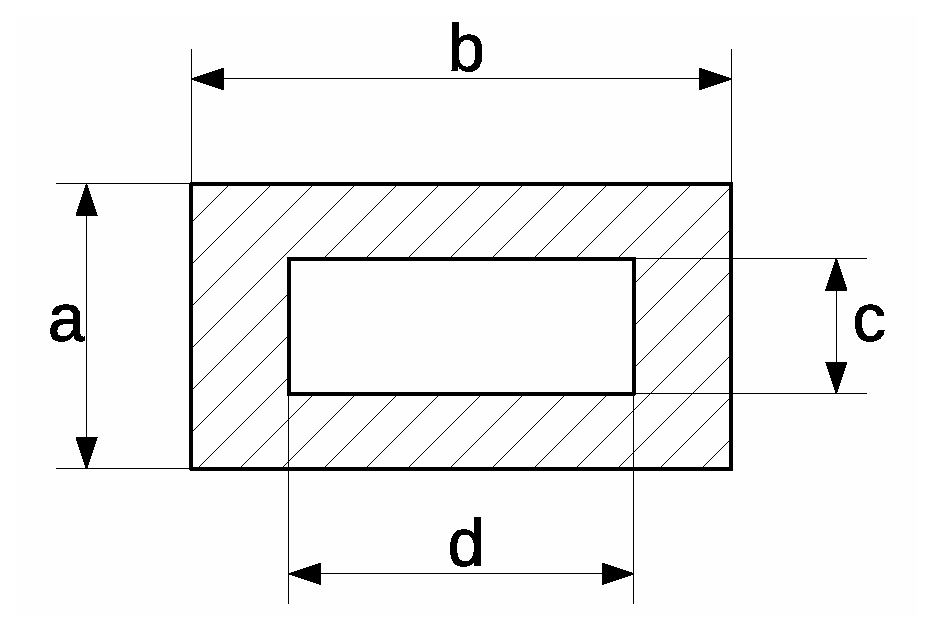
\includegraphics[width=1.0\textwidth]{pictures/Material_budget.eps}
\end{minipage}
\caption{Исходный профиль в CAD-модели (слева) и итоговый профиль в MC-модели.}
\label{fig:geoProfiles}
\end{figure}

Площадь исходного профиля $S_{CAD}$ измеряется стандартной функцией CATIA~v5. Задача заключается в том, чтобы определить размеры $a, b, c, d$ в MC-модели такие, что площадь обоих профилей совпадает, т.е. $S_{CAD} = S_{MC}$. Пользователь может выбрать внешние размеры $a$ и $b$, например так, чтобы они совпадали с габаритами исходного профиля. Очевидно, $S_{MC} = ab - cd$. Пусть $c = ka$ и $d = kb$. Тогда $S_{CAD} = S_{MC} = ab - ka \cdot kb = ab(1 - k^2)$. Отсюда $1 - k^2 = \frac{S_{CAD}}{ab}$ и $k = \sqrt{1 - \frac{S_{CAD}}{ab}}$. Отсюда вычисляются $c$ и $d$.
